\label{sec:1_2_problem_statement}

\begin{comment}
In a short and precise way, state what your research is about in this thesis. It can be in the form of a (set of) research questions, goals/aims, or objectives (or a mix) - but it should clearly state what the problems or challenges you are addressing.

Alternatively, one can state a research hypothesis, but if so, it should follow the rules of what a hypothesis is. A hypothesis is a statement that introduces a research question and proposes an expected result. It is an integral part of the scientific method that forms the basis of scientific experiments. Therefore, you need to be careful and thorough when building your hypothesis, following the “rules”.
\end{comment}

\section{Problem statement}

% Intro
For machine learning and computer vision to be truly trustworthy, they will need to be understood. Researchers need to understand the inner workings of the model to improve it and discover biases in the dataset. Users and domain experts utilizing the models need to have trust in the model predicting accurately while using useful features when evaluating. The models should be able to achieve \gls{sota} performance, without sacrificing interpretability and explainability in what they evaluate when predicting. 

% What this is and How I want to do it
In this thesis, the goal is to explore the roam of visual and linguistic understanding.
The visual knowledge will come from a \gls{cnn} that learns features in images. An \gls{rnn} \cite{rumelhartLearningRepresentationsBackpropagating1986, choLearningPhraseRepresentations2014, sutskeverSequenceSequenceLearning2014, bahdanauNeuralMachineTranslation2016} or transformer is used to extract linguistic information from open-ended questions and answers in natural language, taken from a \gls{vqa} dataset. A backward pass that looks for large gradients through layers of the \gls{cnn} will be used to choose locally faithful words to caption the image in an explainable way. 



% Questions to be answered
The main topics that will be explored to reach the research goal are: 
\begin{itemize}
    \item Does an explainable image caption model improve its answers when trained on a \gls{vqa} dataset?
    \item With only the explaining model choosing the captions, will the output be more intuitive for humans?
    \item Are the explanations, both captions, and answers from open-ended questions locally faithful to the underlying \gls{cnn} model?
    \item If there is enough time during this thesis, it would be an interesting task to see if the image caption and \gls{vqa} will perform better when using transfer learning  on a language model pretrained on a large language dataset. 
\end{itemize}

% What is the result
With these research questions answered, this thesis will be one step closer to an explanatory model that can give insight into how models understand broad concepts in vision and language. This knowledge can be used to make computers understand a more complex worldview and help humans understand what it sees and value.

\subsection{Proposed architecture}
Figure \ref{fig:architecture_proposal} shows how the data flow in the proposed method can work. It closely follows the \gls{flex} \cite{wickramanayakeFLEXFaithfulLinguistic2019} architecture proposed by Wickramanayake et al. It consists of a \gls{cnn} that extracts visual information and a 2-layered \gls{lstm} \cite{hochreiterLongShorttermMemory1997} \gls{rnn} that combine linguistic information with extracted visual features. The reason why this architecture is relevant for this thesis is that it uses a backward pass to find locally accurate visual features, which are then used to give an image caption that describes what visual features actually were important to the classification and captioning of the image. This makes the architecture useful as a starting point for this thesis and can be adapted to use \gls{vqa} datasets as linguistic input, to make it possible to ask questions regarding the classification of images and predictions. 

% Explain the proposed data flow / architecture 
    % Training
    % CNN
During training the proposed architecture takes an image and its corresponding questions and answers from the \gls{vqa} dataset. The images are fed through a \gls{cnn}-network, which can be pretrained on a larger dataset, like ImageNet \cite{dengImageNetLargeScaleHierarchical2009}. This is because the explaining method utilizes feature maps in each layer of the \gls{cnn}, so it is agnostic on what type of \gls{cnn} it is and what dataset it is trained on earlier. The \gls{cnn} predicts a class of what it sees in the image, and with a backward pass, finds important feature maps in each  convolutional layer. Each feature in the set of important feature maps gets associated with a word and stored in a relevance vector. This process is done by computing a co-occurrence score between each word in the ground truth caption and the feature. The feature with the highest co-occurrence score gets linked with that feature. 

    % LSTM
The \glspl{lstm} gets trained by feeding each word in the ground truth caption into the first layer, alongside the hidden state of the \gls{lstm}. This is used to compute the next state, which gets concatenated with important visual features, and is input to the second, and last, \gls{lstm}-layer. 
The output from the second \gls{lstm}-layer is encoded to vocabulary space that is used to make a conditional probability distribution that later will be used to calculate the probability for predicting that word, given the given image features. 

    % Testing
During prediction, the architecture takes an image and an optional question as input. The \gls{cnn} extracts important features in the layers, which get fed into the \gls{lstm}. Important feature maps from the \gls{cnn} are also used to calculate the relevance vector between features in the image and words. The \gls{lstm} uses this relevance vector, alongside important decision-relevant features from the image to predict a word. This word prediction is repeated until the stop word is predicted. 

If no question is input to the algorithm during prediction, the model will use the most accurate predicted answer caption that describe the image as a whole as a caption for the image. On the other hand, if a question is submitted alongside the image, the \gls{lstm} will generate captions that answer the question asked, and then choose the most decision-relevant answer as the caption. 



% Data flow
\begin{figure}[htb]
    \centering
    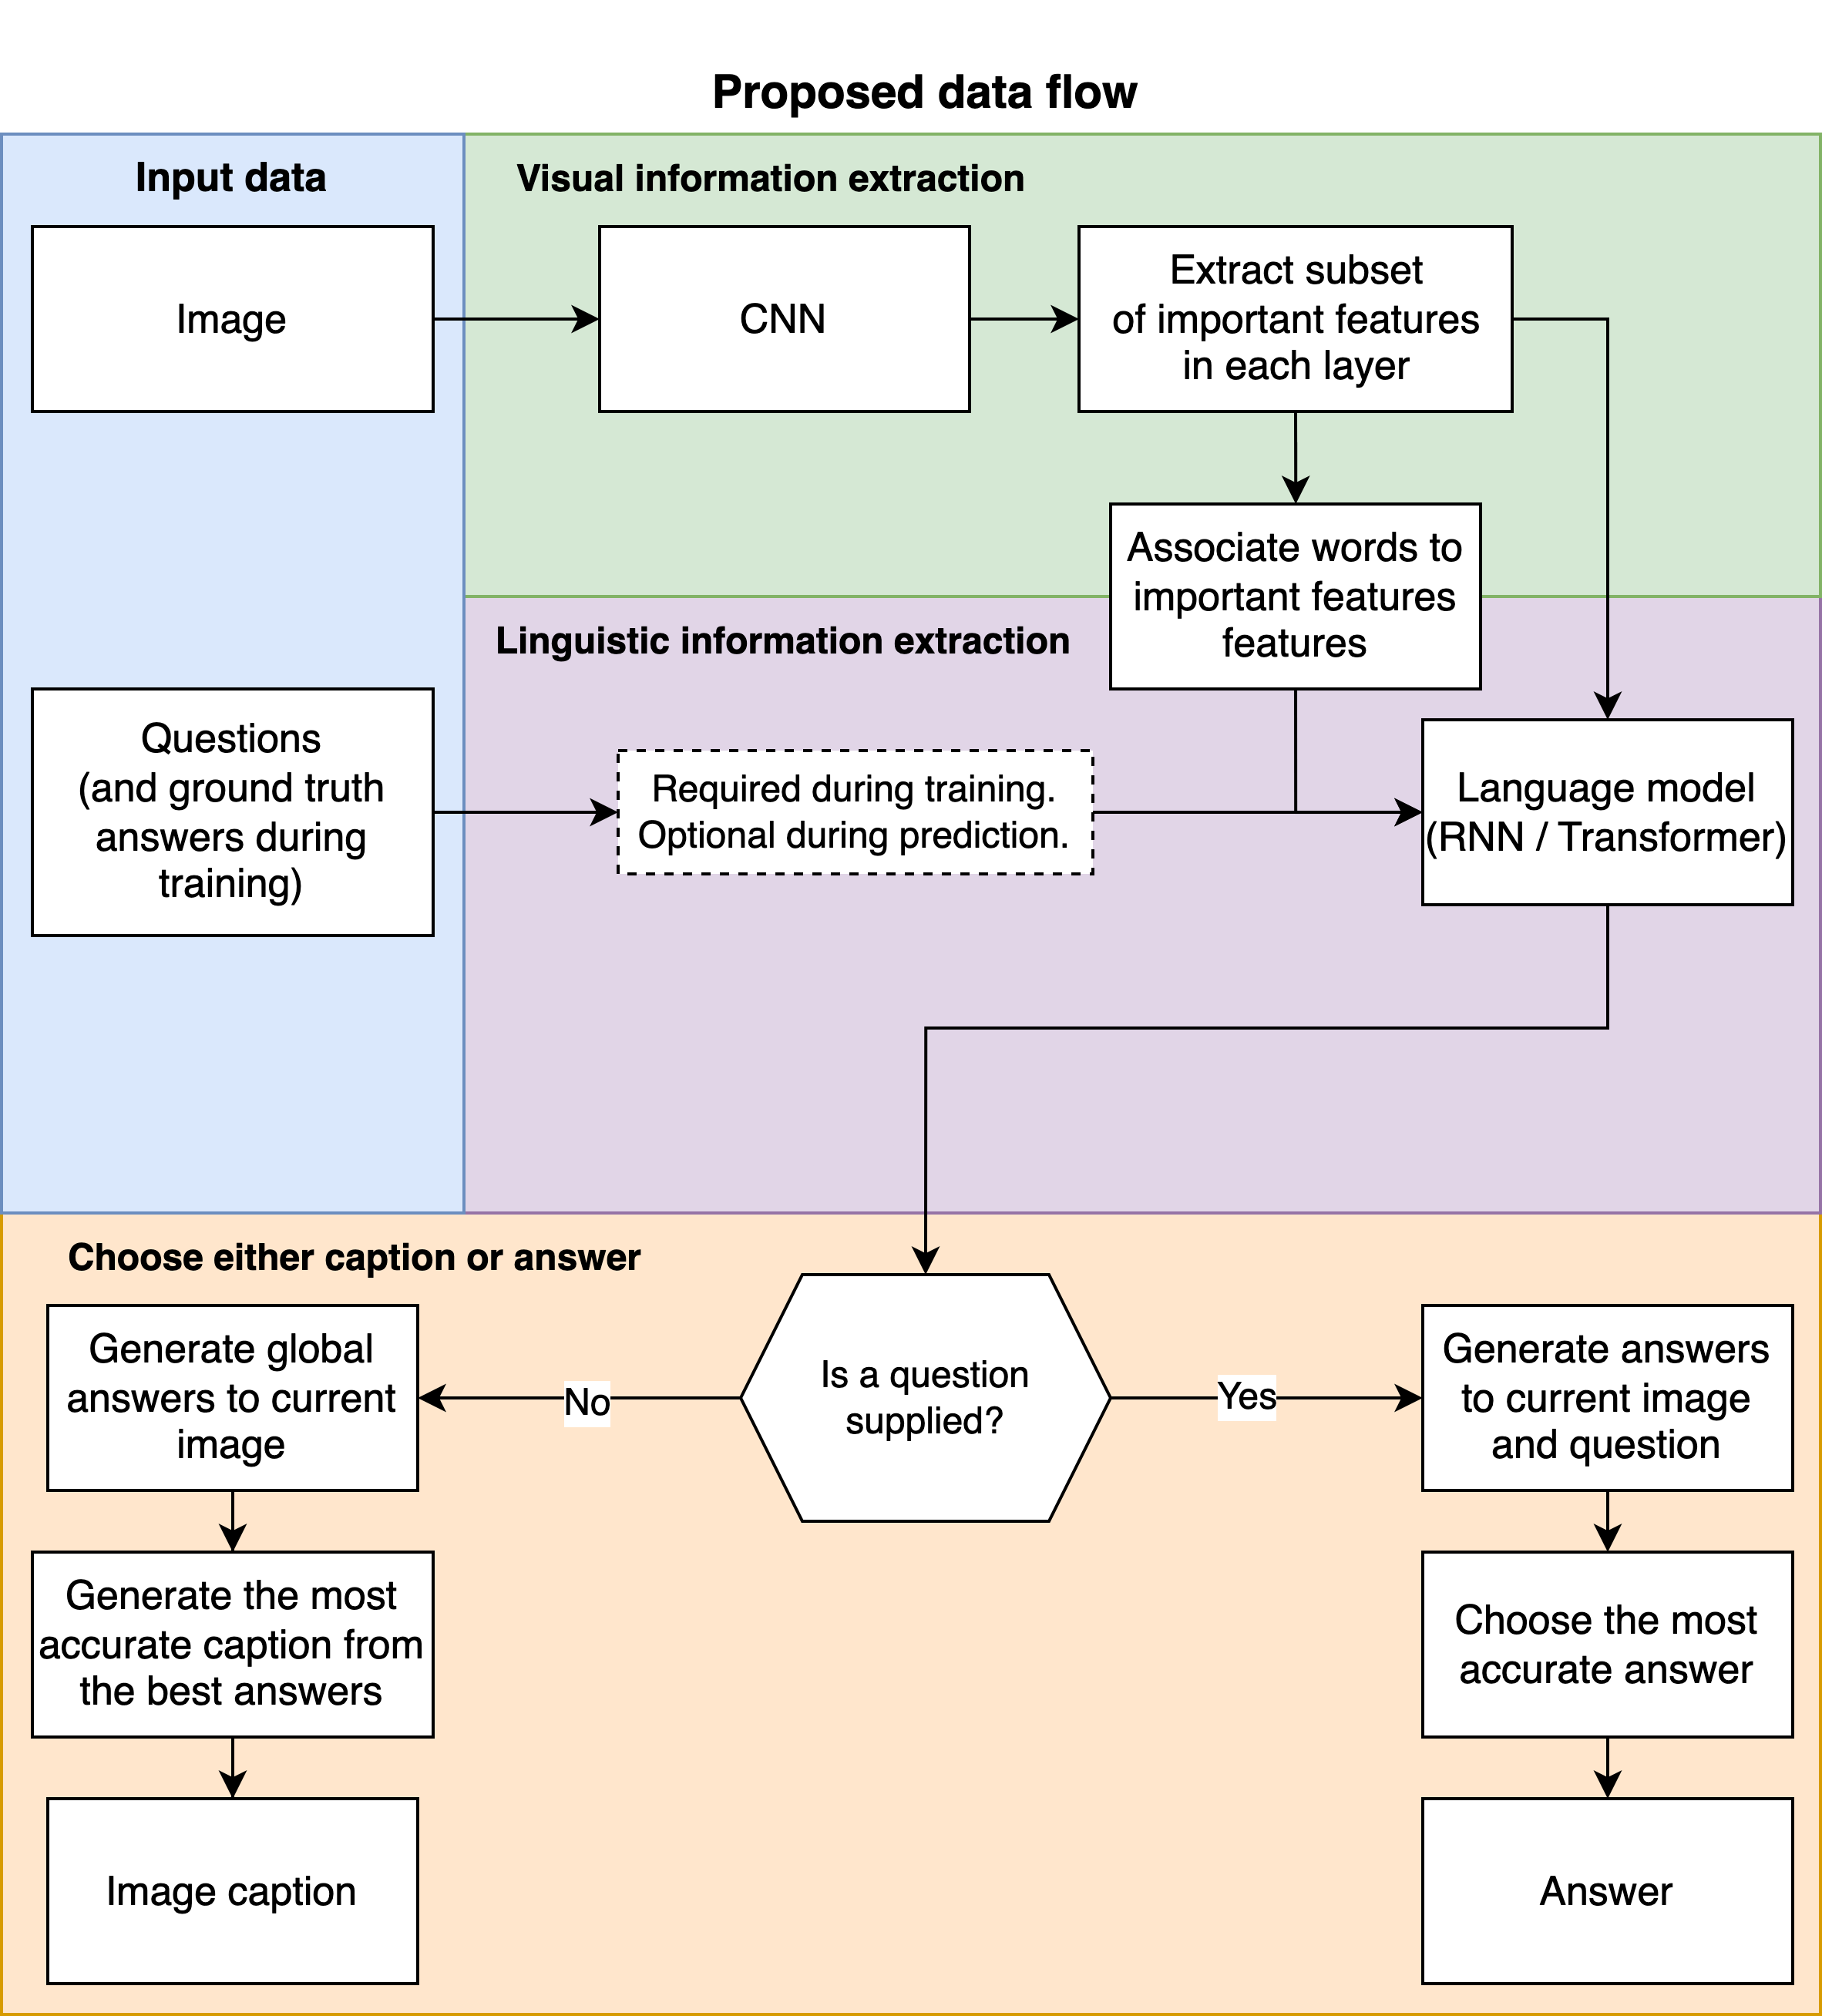
\includegraphics[width=12cm]{images/architecture_proposal.png}
    \caption{Proposal of the data flow and components that will be explored in this thesis.}
    \label{fig:architecture_proposal}
\end{figure}